\begin{exercice*}
    Sur cette figure :
    \begin{itemize}
        \item Les points $O$, $M$, $N$ sont alignés dans cet ordre.
        \item Les points $O$, $V$, $S$ sont alignés dans cet ordre.
    \end{itemize}
    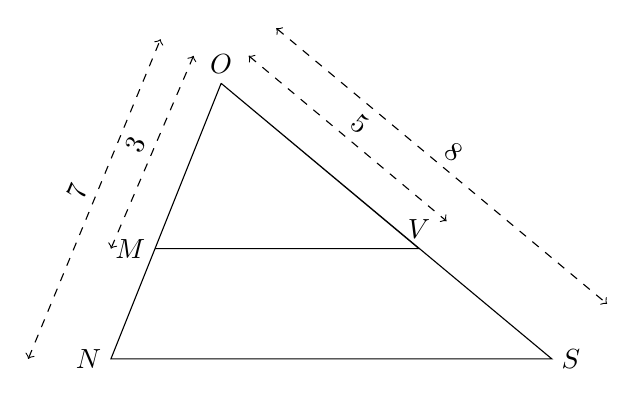
\begin{tikzpicture}[scale=0.7]
        % \draw[help lines, color=black!30, dashed] (0,0) grid (8,12);        
        \coordinate[label=above:$O$] (O) at (4,6);
        \coordinate[label=left:$M$] (M) at (2.8,3);
        \coordinate[label=left:$N$] (N) at (2,1);
        \coordinate[label=above:$V$] (V) at (7.59,3);
        \coordinate[label=right:$S$] (S) at (10,1);
        \draw(O)--(N)--(S)--(O)--(V)--(M);
        \draw[<->, dashed] (2,3)--node[sloped,above] {\Lg{3}} (3.5,6.5);
        \draw[<->, dashed] (0.5,1)--node[sloped,above] {\Lg{7}} (2.9,6.8);
        \draw[<->, dashed] (4.5,6.5)--node[sloped,above] {\Lg{5}} (8.09,3.5);
        \draw[<->, dashed] (5,7)--node[sloped,above] {\Lg{8}} (11,2);
    \end{tikzpicture}

    \begin{enumerate}
        \item Calculer et comparer les proportions $\dfrac{OM}{ON}$ et $\dfrac{OV}{OS}$.
        \item Justifier la position relative des 
        
        droites $(NS)$ et $(MV)$.
    \end{enumerate}
    

\end{exercice*}
\begin{corrige}
    %\setcounter{partie}{0} % Pour s'assurer que le compteur de \partie est à zéro dans les corrigés
    % \phantom{rrr}

    \begin{enumerate}
        \item $\dfrac{OM}{ON}=\dfrac{3}{7}=\dfrac{24}{56}$ et $\dfrac{OV}{OS}=\dfrac{5}{8}=\dfrac{35}{56}$.
        
        Donc $\dfrac{OM}{ON}\neq\dfrac{OV}{OS}$.
        \item On constate que $\dfrac{OM}{ON}\neq\dfrac{OV}{OS}$, l'une des conclusions du théorème de Thalès est contredite, 
        d'après la contraposée de ce théorème, les droites $(MV)$ et $(NS)$ ne sont donc pas parallèles.
    \end{enumerate}

\end{corrige}

